\documentclass[./\jobname.tex]{subfiles}
\begin{document}
%
\def\codeFolderName{DSM_DAC_toplevel_design_starting_point}
\def\codeFileName{}
\def\codeFolderNameB{}
%
\chapter{DAC}
%
\section{Einleitung}
%
Um die entwickelte Logik in ein reales System einzubetten, müssen einige Aufgaben erledigt werden:
%
\begin{itemize}
	\item Geräteauswahl
	\item Pinbelegung
	\item Fertige Module (IP) hinzufügen
	\item Toplevel-Routing
	\item Top-Level-Simulation
	\item Synthese des Projekts in die Zielhardware
	\item Testbench Überprüfung
	\item Validierung (wenn möglich)
\end{itemize}
%
\section{Top-Level Design}
%
In \autoref{fig: Simulink Implementierung} ist das Top-Level Design ersichtlich. Die Verbindungen der Clock (\enquote{clk50m}) und des Reset Eingangs (\enquote{rst\_n}) wurden der Übersichtlichkeit nicht eingezeichnet.
%
\begin{figure}[H]
	\centering
	\noindent\adjustbox{max width=\textwidth}{%falls größer als \textwidth, wird das Bild verkleinert
		%trim option's parameter order: left bottom right top
		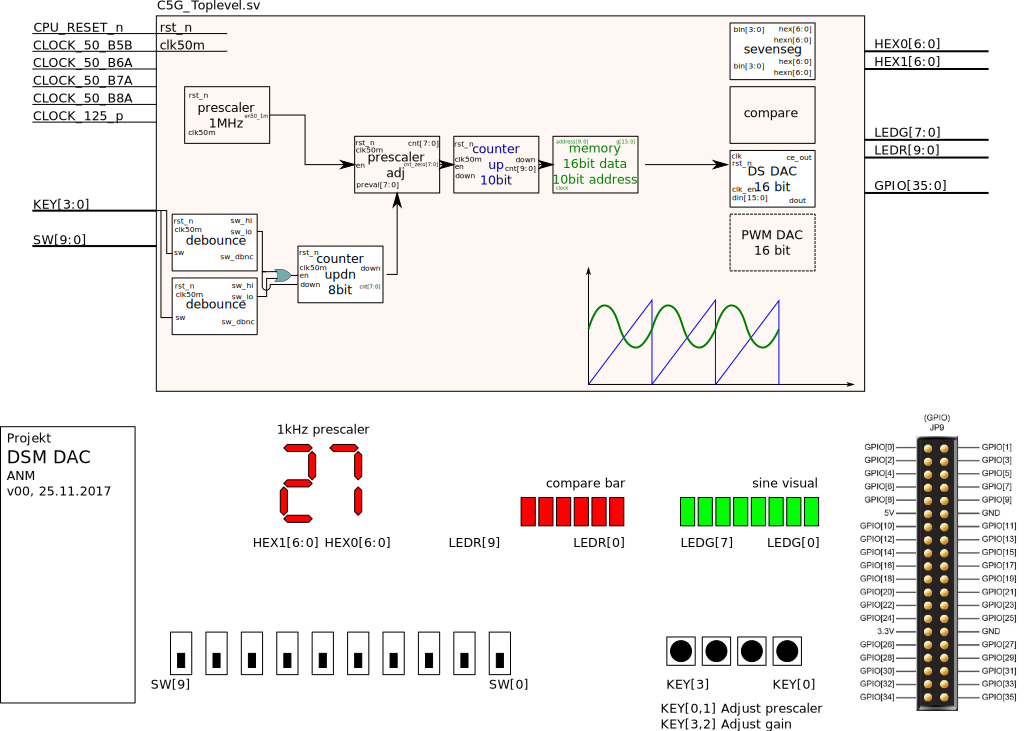
\includegraphics[width=1\textwidth,page=1]{./../code/\codeFolderName\codeFolderNameB/doc/DSM_DAC_board_v0.pdf}
	}
	\unterschrift{Top-Level Design}{Mitterbacher Andrè und eigene Erweiterung}{}
	\label{fig: Simulink Implementierung}
\end{figure}
%
In \autoref{fig: toplevel.pdf} ist das im Quartus implementierte Top-Level Design ersichtlich.
%
\begin{figure}[H]
	\centering
	\noindent\adjustbox{max width=\textwidth}{%falls größer als \textwidth, wird das Bild verkleinert
		%trim option's parameter order: left bottom right top
		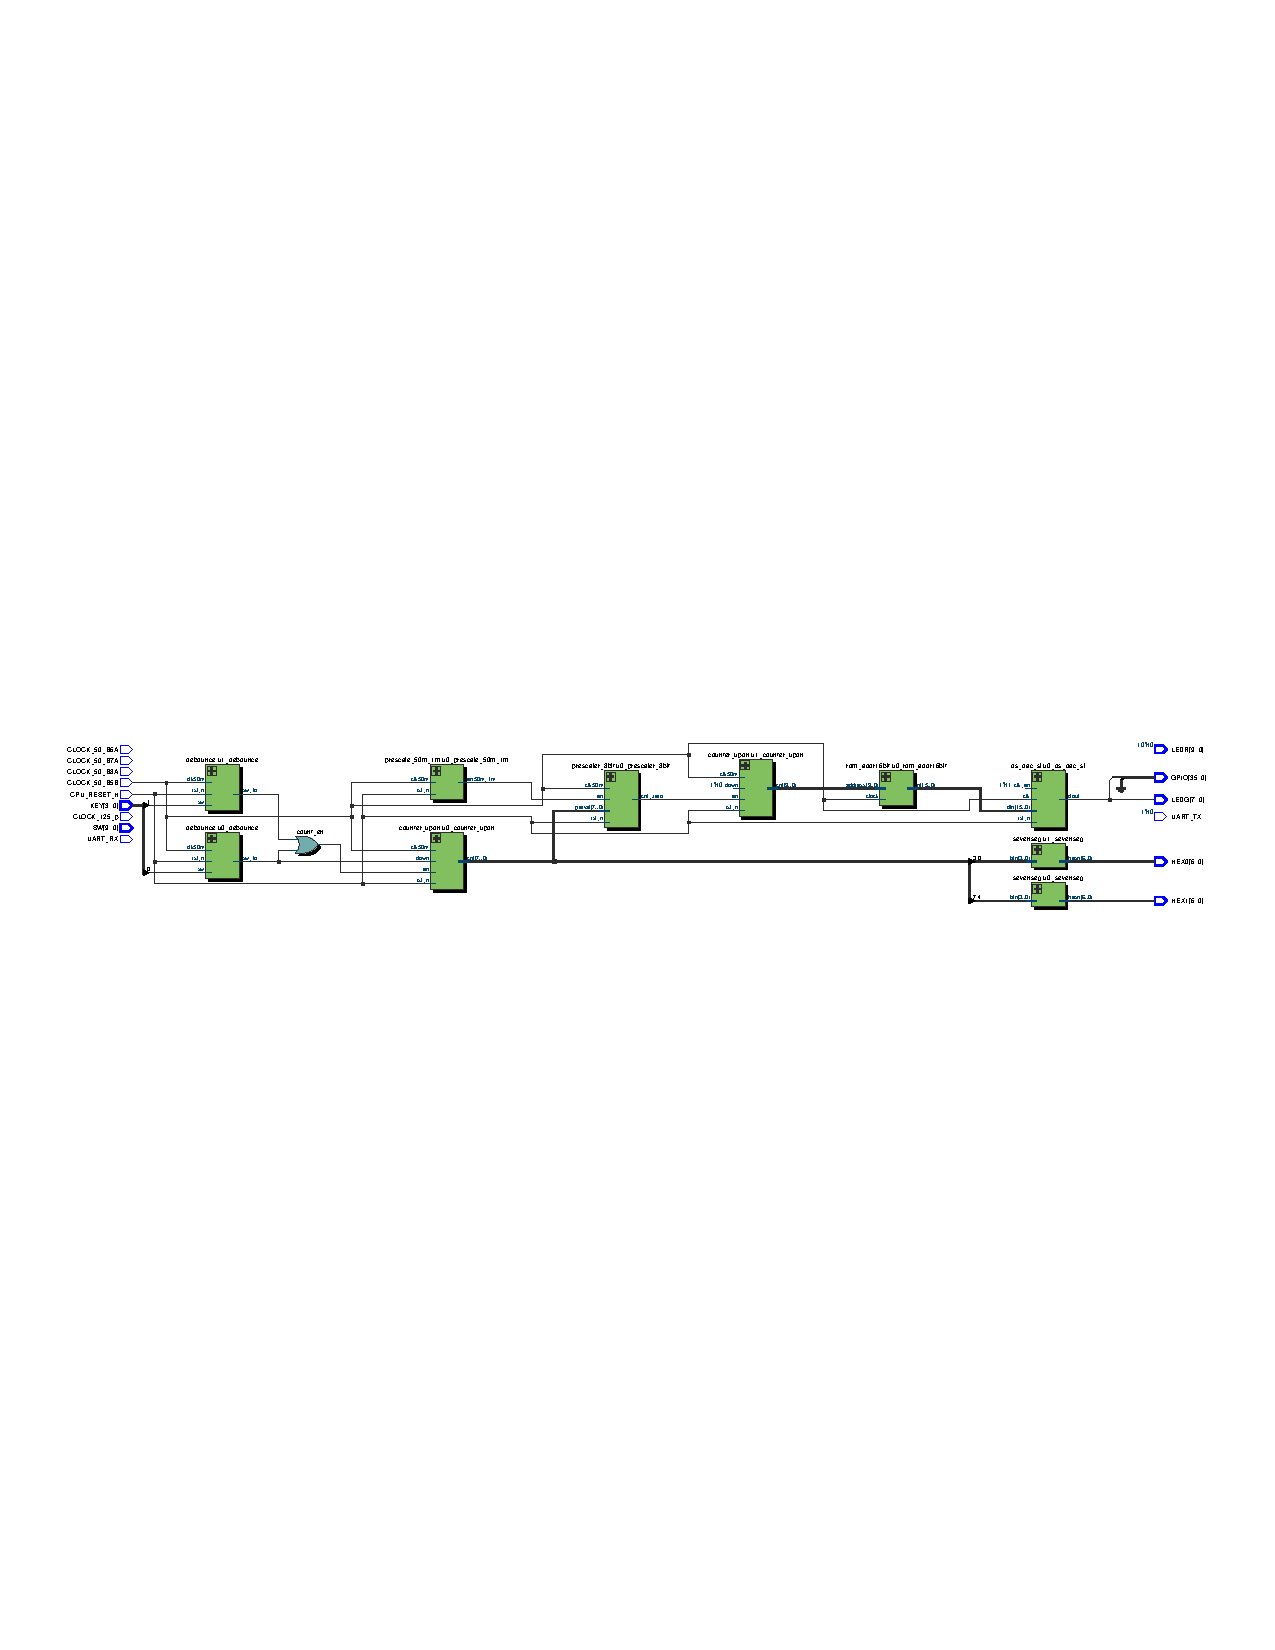
\includegraphics[width=1\textwidth,page=1]{./../code/\codeFolderName\codeFolderNameB/doc/toplevel.pdf}
	}
	\unterschrift{Top-Level Design}{eigene Ausarbeitung}{}
	\label{fig: toplevel.pdf}
\end{figure}
%
\section{Toplevel Design und Simulation}
%
In \autoref{lst: toplevel sim code} ist das Toplevel Design ersichtlich.
%
\lstinputlisting[language=Verilog,label={lst: toplevel sim code}, caption=Toplevel Design]{./../code/\codeFolderName\codeFolderNameB/src/toplevel_c5g_led_switch_7segx2_gpio_uart.sv}
%
In \autoref{lst: toplevel sim tb} ist der Code der Testbench ersichtlich. 
%
\lstinputlisting[language=Verilog,label={lst: toplevel sim tb}, caption=Testbench]{./../code/\codeFolderName\codeFolderNameB/sim/tb_toplevel_c5g_led_switch_7segx2_gpio_uart.sv}
%
\autoref{fig: wave.PNG} zeigt den simulierten Sinus.
%
\begin{figure}[H]
	\centering
	\noindent\adjustbox{max width=\textwidth}{%falls größer als \textwidth, wird das Bild verkleinert
		%trim option's parameter order: left bottom right top
		\includegraphics[width=1\textwidth,page=6]{./../code/\codeFolderName\codeFolderNameB/doc/wave.PNG}
	}
	\unterschrift{Sinus Verifikation in der Simulation}{eigene Ausarbeitung}{}
	\label{fig: wave.PNG}
\end{figure}
%
%\lstinputlisting[language=Verilog,label={lst:tb_counter_updn}, caption=Testbench für den \glsentryshort{dac}]{./../code/\codeFolderName\codeFolderNameB/sim/tb_\codeFileName.sv}
%
\section{Bench Verifikation}
%
Der Bitstream wird mit einem Tiefpassfilter erster Ordnung gefiltert (\autoref{fig: Tiefpassfilter}).
%
\begin{align}
f_{g}&= \frac{1}{2 \cdot \pi \cdot R \cdot C}
\end{align}
%
Mit \(C=1~nF\) und \(R=10~k\Omega\) folgt für \(f_{g}\)
%
\begin{align}
	f_{g}&= 15,91~kHz
\end{align}
%
Der erzeugte Sinus hat eine Frequenz von \(f_{max}=976,56~Hz\) unter der Annahme, dass der Prescaler eine Frequenz von \(10~MHz\) und der gespeicherte Sinus \(1024\) Werte für eine Periode hat.
%
\begin{align}
f_{max}&=\frac{10^{6}~Hz}{1024}\\
&=976,56~Hz
\end{align}
%
\def\bildA{false}
\begin{figure}[H]
	\centering
	\noindent\adjustbox{max width=\textwidth}{%falls größer als \textwidth, wird das Bild verkleinert
		\subfile{./img/tikz/tiefpass.tex}
	}
	\unterschrift{Tiefpass erster Ordnung}{eigene Ausarbeitung}{}
	\label{fig: Tiefpassfilter}
\end{figure}
%
In \autoref{fig: oszi_dutytrack} ist der generierte Sinus dargestellt. Channel 1 zeigt die gemessene Spannung über die Zeit am Ausgang des Tiefpassfilters. Channel 2 zeigt den Bitstream am Ausgang des GPIO[0]. Die Funktion F1 zeigt das Tracking des Dutycycles. Durch das Ändern des Speichers lässt sich die Art des Ausgangsbitstromes und somit der generierten Spannung beliebig wählen. \autoref{fig: ramp.png} zeigt eine generierte Sägezahnspannung, \autoref{fig: triangle.png} zeigt eine generierte Dreiecksspannung und \autoref{fig: square.png} zeigt eine generierte Rechteckspannung.
%
\begin{figure}[H]
	\centering
	\noindent\adjustbox{max width=\textwidth}{%falls größer als \textwidth, wird das Bild verkleinert
		%trim option's parameter order: left bottom right top
		\includegraphics[width=1\textwidth,page=6]{./../code/\codeFolderName\codeFolderNameB/doc/oszi_dutytrack.png}
	}
	\unterschrift{Sinus Verifikation}{eigene Ausarbeitung}{}
	\label{fig: oszi_dutytrack}
\end{figure}
%
\autoref{fig: spectrum_sin} zeigt das Spektrum des erzeugten Sinussignals mit Prescaler 7. Die Grundschwingung mit \(139~Hz\) hat eine deutlich höhere Amplitude (siehe linke Tabelle) als die erste Oberschwingung mit \(279~Hz\).
%
\begin{figure}[H]
	\centering
	\noindent\adjustbox{max width=\textwidth}{%falls größer als \textwidth, wird das Bild verkleinert
		%trim option's parameter order: left bottom right top
		\includegraphics[width=1\textwidth,page=6]{./../code/\codeFolderName\codeFolderNameB/doc/spectrum_sin.png}
	}
	\unterschrift{Spektrum des Sinussignals}{Hermann Haag}{}
	\label{fig: spectrum_sin}
\end{figure}
%
\begin{figure}[H]
	\centering
	\noindent\adjustbox{max width=\textwidth}{%falls größer als \textwidth, wird das Bild verkleinert
		%trim option's parameter order: left bottom right top
		\includegraphics[width=1\textwidth,page=6]{./../code/\codeFolderName\codeFolderNameB/doc/ramp.png}
	}
	\unterschrift{Sägezahn Verifikation}{eigene Ausarbeitung}{}
	\label{fig: ramp.png}
\end{figure}
%
\begin{figure}[H]
	\centering
	\noindent\adjustbox{max width=\textwidth}{%falls größer als \textwidth, wird das Bild verkleinert
		%trim option's parameter order: left bottom right top
		\includegraphics[width=1\textwidth,page=6]{./../code/\codeFolderName\codeFolderNameB/doc/triangle.png}
	}
	\unterschrift{Dreieck Verifikation}{eigene Ausarbeitung}{}
	\label{fig: triangle.png}
\end{figure}
%
\begin{figure}[H]
	\centering
	\noindent\adjustbox{max width=\textwidth}{%falls größer als \textwidth, wird das Bild verkleinert
		%trim option's parameter order: left bottom right top
		\includegraphics[width=1\textwidth,page=6]{./../code/\codeFolderName\codeFolderNameB/doc/square.png}
	}
	\unterschrift{Rechteck Verifikation}{eigene Ausarbeitung}{}
	\label{fig: square.png}
\end{figure}
%
\end{document}
